\documentclass[varwidth=true, border=2pt]{standalone}
\usepackage{tikz}
\usetikzlibrary{arrows,positioning}
\tikzset{
    %Define standard arrow tip
    >=stealth',
    % Define arrow style
    pil/.style={
           ->,
           thick}
}

\begin{document}
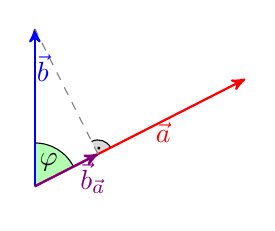
\begin{tikzpicture}
    \draw[fill=gray!30] (27:0.90) -- node[right=-0.28cm, near end] {$\cdot$} (27:1.08)
                        arc (27:117:.18cm);
    \draw[fill=green!30] (0,0) -- (90:.55cm) arc (90:27:.55cm);
    \draw[pil,color=red] (0,0) -- node[right=2pt] {$\vec a$} (27:3cm);
    \draw[pil,color=blue] (0,0) -- node[near end, right=-3pt] {$\vec b$} (90:2cm);

    \draw[pil,color=violet] (0,0) -- node[near start, right=7pt] {$\vec b_{\vec a}$} (27:0.90cm);
    \draw[color=gray, dashed] (27:0.90) -- node[near end, right] {} (90:2cm);

    \draw(60:0.35cm) node {$\varphi$};
  \end{tikzpicture}
\end{document}
